%%
%% Supplementary Information (Additional File 1) for
%% muxvizpy — Application Note for Bioinformatics
%%
%% Single-column standalone document.
%%
\documentclass[11pt,onecolumn]{article}

\usepackage[a4paper,margin=2.2cm]{geometry}
\usepackage{amsmath,amssymb,amsthm}
\usepackage{bbm} % for \mathbbm{1} (indicator / all-ones symbol)
\usepackage{booktabs}
\usepackage{graphicx}
\usepackage{algorithm}
\usepackage{algpseudocode}
\usepackage{xcolor}
\usepackage[round,authoryear]{natbib}
\usepackage[colorlinks=true,allcolors=blue!55!black]{hyperref}
\usepackage{caption}
\captionsetup{font=small,labelfont=bf}

\graphicspath{{Fig/}{media/}}

% Theorem-like environments
\theoremstyle{definition}
\newtheorem{definition}{Definition}
\theoremstyle{remark}
\newtheorem{remark}{Remark}

% "S" prefixes for a supplementary document
\renewcommand{\thesection}{S\arabic{section}}
\renewcommand{\thesubsection}{S\arabic{section}.\arabic{subsection}}
\renewcommand{\thefigure}{S\arabic{figure}}
\renewcommand{\thetable}{S\arabic{table}}
\renewcommand{\thealgorithm}{S\arabic{algorithm}}
\renewcommand{\thedefinition}{S\arabic{definition}}
\renewcommand{\theremark}{S\arabic{remark}}
\renewcommand{\theequation}{S\arabic{equation}}

% Local helpers
\newcommand{\tbd}[1]{\textcolor{blue}{[TBD] #1}}
\newcommand{\mat}[1]{\mathbf{#1}}
\newcommand{\ten}[1]{\boldsymbol{\mathcal{#1}}}
\newcommand{\supra}{\mat{A}}
\newcommand{\R}{\mathbb{R}}
\newcommand{\code}[1]{\texttt{#1}}

% Placeholder box for figures whose benchmark/accuracy results are still pending.
% Swap the whole \placeholderfig line for an \includegraphics once results exist.
\newcommand{\placeholderfig}[2][\linewidth]{%
  \setlength{\fboxsep}{0pt}%
  \fcolorbox{black!35}{black!8}{%
    \parbox[c][0.4\textwidth][c]{#1}{%
      \centering\itshape\color{black!60}%
      [PLACEHOLDER]\\[4pt]#2\\[6pt]%
      \upshape\footnotesize results pending%
    }%
  }%
}

\title{\textbf{Supplementary Information}\\[4pt]
\Large A Probabilistic Ensemble-Based Bayesian Method for Mechanistic GRN Inference}
\author{Francesco Zambelli, Valeria D'Andrea, Manlio De Domenico}
\date{}

\begin{document}
\maketitle

\section{Likelihood Convexity}

To determine whether the likelihood is convex or not with respect to the interaction matrix weights, we compute the Hessian matrix and verify that it is semi-positive definite.

We focus on a single node $i$. Under the Euler-Maruyama discretization, the objective function to minimize (the negative log-likelihood) over $M$ time steps is the sum of squared residuals:

$$ \mathcal{L}(\mathbf{W}_i) = \frac{1}{4D \Delta t} \sum_{k=1}^M (e_{i,k})^2 $$

Where the residual error $e_{i,k}$ at time step $k$ is defined as:

$$ e_{i,k} = x_{i, k} - x_{i, k-1} - \Delta t \Big( -\gamma_i x_{i, k-1} + V_i \sigma(z_{i,k-1}) \Big) $$

And $z_{i,k-1} = \sum_{j} W_{ij} x_{j,k-1}$ is the total input to the sigmoid function.

The first derivative is:
$$ \frac{\partial \mathcal{L}}{\partial W_{ij}} = \frac{1}{2D \Delta t} \sum_{k=1}^M e_{i,k} \frac{\partial e_{i,k}}{\partial W_{ij}} $$

Taking the derivative of the residual $e_{i,k}$ with respect to $W_{ij}$:
$$ \frac{\partial e_{i,k}}{\partial W_{ij}} = - \Delta t \, V_i \, \sigma'(z_{i,k-1}) \, x_{j, k-1} $$

So the gradient is:
$$ \frac{\partial \mathcal{L}}{\partial W_{ij}} = - \frac{V_i}{2D} \sum_{k=1}^M e_{i,k} \, \sigma'(z_{i,k-1}) \, x_{j, k-1} $$

Taking the second derivative, we get the entries of the Hessian matrix:

$$ H_{i,j} = \frac{\partial^2 \mathcal{L}}{\partial W_{ij} \partial W_{il}} = \frac{1}{2D \Delta t} \sum_{k=1}^M \left[ \frac{\partial e_{i,k}}{\partial W_{ij}} \frac{\partial e_{i,k}}{\partial W_{il}} + e_{i,k} \frac{\partial^2 e_{i,k}}{\partial W_{ij} \partial W_{il}} \right] $$

Unpacking each term:
    $$ \frac{\partial e_{i,k}}{\partial W_{ij}} \frac{\partial e_{i,k}}{\partial W_{il}} = \Delta t^2 V_i^2 [\sigma'(z_{i,k-1})]^2 \, x_{j, k-1} \, x_{l, k-1} $$
    
    $$ e_{i,k} \frac{\partial^2 e_{i,k}}{\partial W_{ij} \partial W_{il}} = - \Delta t \, V_i \, e_{i,k} \, \sigma''(z_{i,k-1}) \, x_{j, k-1} \, x_{l, k-1} $$

Combining both terms and factoring out 
$x_{j, k-1} x_{l, k-1}$, the full Hessian matrix element is:

$$ H_{jl} = \frac{V_i}{2D} \sum_{k=1}^M x_{j, k-1} x_{l, k-1} \underbrace{\left[ \Delta t \, V_i \big(\sigma'(z_{i,k-1})\big)^2 - e_{i,k} \, \sigma''(z_{i,k-1}) \right]}_{c_k} $$

In matrix form, the Hessian is $\mathbf{H} = \mathbf{X}^T \mathbf{C} \mathbf{X}$, where $\mathbf{C}$ is a diagonal matrix containing the coefficients $c_k$. 

\begin{equation}
    c_k = \Delta t \, V_i \big(\sigma'(z_{i,k-1})\big)^2 - e_{i,k} \, \sigma''(z_{i,k-1})
    \label{eq::ck}
\end{equation}

For the likelihood $\mathcal{L}$ to be strictly convex, the Hessian $\mathbf{H}$ must be Positive Semi-Definite (PSD) everywhere. This requires that the coefficient $c_k \ge 0$ for all time steps $k$.
Looking at \ref{eq::ck}, we can notice that the first term is always positive, while the second one can be negative, given that the second derivative of the sigmoid changes sign with respect to the sign of the argument.

This fact does not allow to be sure that a simple gradient descent algorithm can safely converge to the global minimum of the likelihood function. 

\section{Parameter Indistinguishability}

\subsection{Equilibrium Scaling Degeneracy ($\gamma_i \sim V_i$)}

Near dynamic equilibrium or steady state, the drift vanishes ($\Delta x_i(t) / \Delta t \approx 0$), yielding the stationary expectation:

$$x_i^* = \frac{V_i}{\gamma_i} \sigma\left( \sum_j W_{ij} x_j^* \right)$$

If both degradation $\gamma_i$ and transcription scale $V_i$ are multiplied by a scale factor $c > 0$:

$$\gamma_i \mapsto c \gamma_i, \quad V_i \mapsto c V_i \implies \frac{cV_i}{c\gamma_i} = \frac{V_i}{\gamma_i}$$

Thus, the stationary expression $x_i^*$ is invariant to uniform scaling of $(\gamma_i, V_i)$. In data lacking strong non-equilibrium transients, MCMC proposals along the ridge $\gamma_i = c V_i$ produce identical steady-state predictions.

\subsection{Sigmoid Saturation Degeneracy ($|m_i| \gg 1$)}

The derivative of the drift term with respect to an edge weight $W_{ij}$ is:

$$\frac{\partial f_i}{\partial W_{ij}} = V_i \frac{\partial \sigma(m_i)}{\partial m_i} x_j = V_i \sigma(m_i)\left(1 - \sigma(m_i)\right) x_j$$

When total regulatory input $|m_i| = \left|\sum_j W_{ij} x_j\right|$ is large, the sigmoid saturates ($\sigma(m_i) \to 0$ or $1$). In this saturated regime, the gradient vanishes:

$$\lim_{|m_i| \to \infty} \sigma(m_i)(1 - \sigma(m_i)) = 0$$

Consequently, once an edge $W_{ij}$ drives gene $i$ into saturation, further changes to $W_{ij}$ or addition of new edges $W_{ik}$ produce virtually zero change in log-likelihood ($\Delta S \approx 0$), causing edge misinference.

\subsection{Multiplicative Linear Indeterminacy ($V_i W_{ij} = \text{const}$)}

When regulatory inputs are small ($|m_i| \lesssim 1$), the sigmoid operates in its linear regime ($\sigma(m_i) \approx \frac{1}{2} + \frac{1}{4} m_i$). The drift simplifies to:

$$f_i(x) \approx -\gamma_i x_i + \frac{1}{2} V_i + \frac{1}{4} V_i \sum_j W_{ij} x_j$$

In this linear regime, scaling $V_i \mapsto \alpha V_i$ while inversely scaling edge weights $W_{ij} \mapsto \alpha^{-1} W_{ij}$ leaves the effective interaction strength $V_i W_{ij}$ unchanged, introducing a multiplicative degeneracy between node parameters and edge weights.

\section{Generative Model and Synthetic Data Setup}

To validate the inference framework, we generated synthetic data using a continuous-time Stochastic Differential Equation (SDE) model. The underlying ground-truth network topologies were generated as directed scale-free graphs using the Price model (Barabási-Albert with directed preferential attachment) with an out-degree parameter $m=2$. This ensures the presence of highly connected ``master regulators,'' which are characteristic of biological gene regulatory networks. The true edge weights $W_{ij}$ were uniformly sampled from the disjoint intervals $[-2.0, -0.5] \cup [0.5, 2.0]$ to guarantee that the interactions have a non-negligible biological effect (either activating or repressing) while avoiding vanishingly small weights.

The dynamics of the $N$ nodes were simulated using the following non-linear SDE with Cox-Ingersoll-Ross (CIR) multiplicative noise:
\begin{equation}
    dx_i(t) = \left( -\gamma_i x_i(t) + V_i \sigma\left(\sum_{j=1}^N W_{ij} x_j(t)\right) \right) dt + \sqrt{2 D_i x_i(t)} dW_i(t)
\end{equation}
where $\sigma(\cdot)$ is the standard logistic sigmoid function. For the baseline homogeneous experiments, the kinetic parameters were set globally to $\gamma = 0.5$, $V = 2.0$, and $D = 0.1$.

Trajectories were simulated using the Euler-Maruyama numerical integration scheme with a highly resolved simulation step $\Delta t_{sim} = 0.01$. The continuous trajectories were then subsampled at larger measurement intervals $\Delta t_{meas}$ (e.g., $0.05$ to $0.5$) to replicate the sparsity of real-world experimental time-series. Transient trajectories were generated by initializing the system at uniformly random states $x_i(0) \sim U(0.1, 1.0)$ and sampling during the initial relaxation phase, whereas stationary trajectories were sampled after the system had reached stochastic equilibrium.

\section{Exact Analytical Transition Moments (Itô Isometry)}

The Euler-Maruyama discretization, while computationally simple, is mathematically guaranteed to become unstable at large measurement intervals ($\Delta t$), failing to capture the exponential relaxation of the degradation term and incorrectly modeling the variance. To overcome this, we derive the exact analytical transition moments under a zero-order hold assumption, where the regulatory input $m_i(t) = \sum W_{ij} x_j(t)$ is assumed constant over the interval $\Delta t$.

Under this assumption, the SDE for node $i$ reduces to a strictly linear CIR process:
\begin{equation}
    dx_t = (-\gamma x_t + b) dt + \sqrt{2D x_t} dW_t
\end{equation}
where $b = V \sigma(m_i(t))$. We define the steady-state asymptote as $\mu_\infty = b / \gamma$.

The exact expected mean $\mathbb{E}[x_{t+\Delta t} \mid x_t]$ is the solution to the deterministic ODE part:
\begin{equation}
    \mu(t+\Delta t) = \mu_\infty + (x_t - \mu_\infty)e^{-\gamma \Delta t}
\end{equation}

To find the exact accumulated variance, we apply Itô's Isometry. The variance of the integrated stochastic process over $[0, \Delta t]$ is:
\begin{equation}
    \text{Var}(x_{t+\Delta t} \mid x_t) = \mathbb{E}\left[ \int_0^{\Delta t} e^{-2\gamma(\Delta t - s)} 2D \cdot \mathbb{E}[x_s \mid x_t] ds \right]
\end{equation}
Substituting the exact expected mean $\mathbb{E}[x_s \mid x_t]$ into the integral and evaluating it yields the exact closed-form solution:
\begin{equation}
    \text{Var} = \frac{2D}{\gamma} (x_t - \mu_\infty) (e^{-\gamma \Delta t} - e^{-2\gamma \Delta t}) + \frac{D \mu_\infty}{\gamma} (1 - e^{-2\gamma \Delta t})
\end{equation}
This formula correctly collapses to the Euler-Maruyama variance $2D x_t \Delta t$ as $\Delta t \to 0$, and saturates to the finite steady-state variance $D \mu_\infty / \gamma$ as $\Delta t \to \infty$.

\section{Evaluation Metrics Formulation}

Because the inference produces a posterior ensemble rather than a single point-estimate, we evaluate the structural recovery using probabilistic metrics based on the marginal edge probability $p_{ij}$, which is the fraction of MCMC sweeps in which the edge $i \to j$ exists. The Area Under the Receiver Operating Characteristic (AUROC) and Precision-Recall Curve (AUPRC) were calculated by thresholding $p_{ij}$ directly, bypassing binary MAP predictions.

To evaluate the quantitative weights without being penalized by parameter scaling degeneracy (as discussed in S2), we utilized ranking metrics to compare the inferred expected weights $\bar{W}_{ij}$ against the true weights $W^{true}_{ij}$.
The \textbf{Rank-Biased Overlap (RBO)} was used to quantify the agreement between the top-weighted regulations (e.g., the master regulators). For two ranked lists of edges, RBO is defined as:
\begin{equation}
    \text{RBO} = (1 - p) \sum_{d=1}^E p^{d-1} A_d
\end{equation}
where $A_d$ is the intersection size of the two lists at depth $d$, and $p$ is a top-weighting parameter (set to $p=0.9$).

For the perturbation analysis, where the goal is to predict the downstream steady-state $x_j$ after a knockout, we evaluate the ensemble's predictive power using a \textbf{Kernel Density Estimation (KDE) log-likelihood}. We construct a probability density function $f(x)$ from the ensemble of predicted steady-states using a Gaussian kernel, and evaluate the likelihood of the true biological steady-state $x^{true}$ under this density:
\begin{equation}
    \text{LL}_{KDE} = \log f(x^{true}) = \log \left( \frac{1}{S} \sum_{s=1}^S \mathcal{N}(x^{true} \mid x^{(s)}, h^2) \right)
\end{equation}
where $S$ is the number of ensemble samples and $h$ is the bandwidth chosen via Scott's rule.

\section{Application to the DREAM4 \textit{In Silico} Benchmark}

To evaluate the boundary conditions of our inference framework, we applied the methodology to the DREAM4 \textit{in silico} network challenge (10-node dataset). The DREAM4 data is generated using a highly heterogeneous thermodynamic ODE model, featuring gene-specific transcription, translation, and degradation rates, along with complex noise profiles.

As discussed in the main text, our Bayesian SDE inference engine explicitly enforces a global parameter constraint ($\theta = \{\gamma, V, D\}$ shared across all nodes) to prevent parametric overfitting and force the structural recovery of the network. While this constraint is highly effective for data generated from stochastic non-linear SDEs, it creates a fundamental model mismatch when applied to the highly heterogeneous DREAM4 generative process. 

Because the homogeneous SDE struggles to absorb the massive variance in gene-specific kinetic rates present in the DREAM4 data, the inference engine under-fits the heterogeneous dynamics, leading to degraded structural recovery (see Fig.~\ref{fig:dream4}). This result highlights a critical boundary condition of our approach: the global parameter constraint, while necessary for preventing overfitting in highly sparse stochastic regimes, assumes a degree of kinetic homogeneity that may not hold in all biological or synthetic settings.

\begin{figure*}[h!]
    \centering
    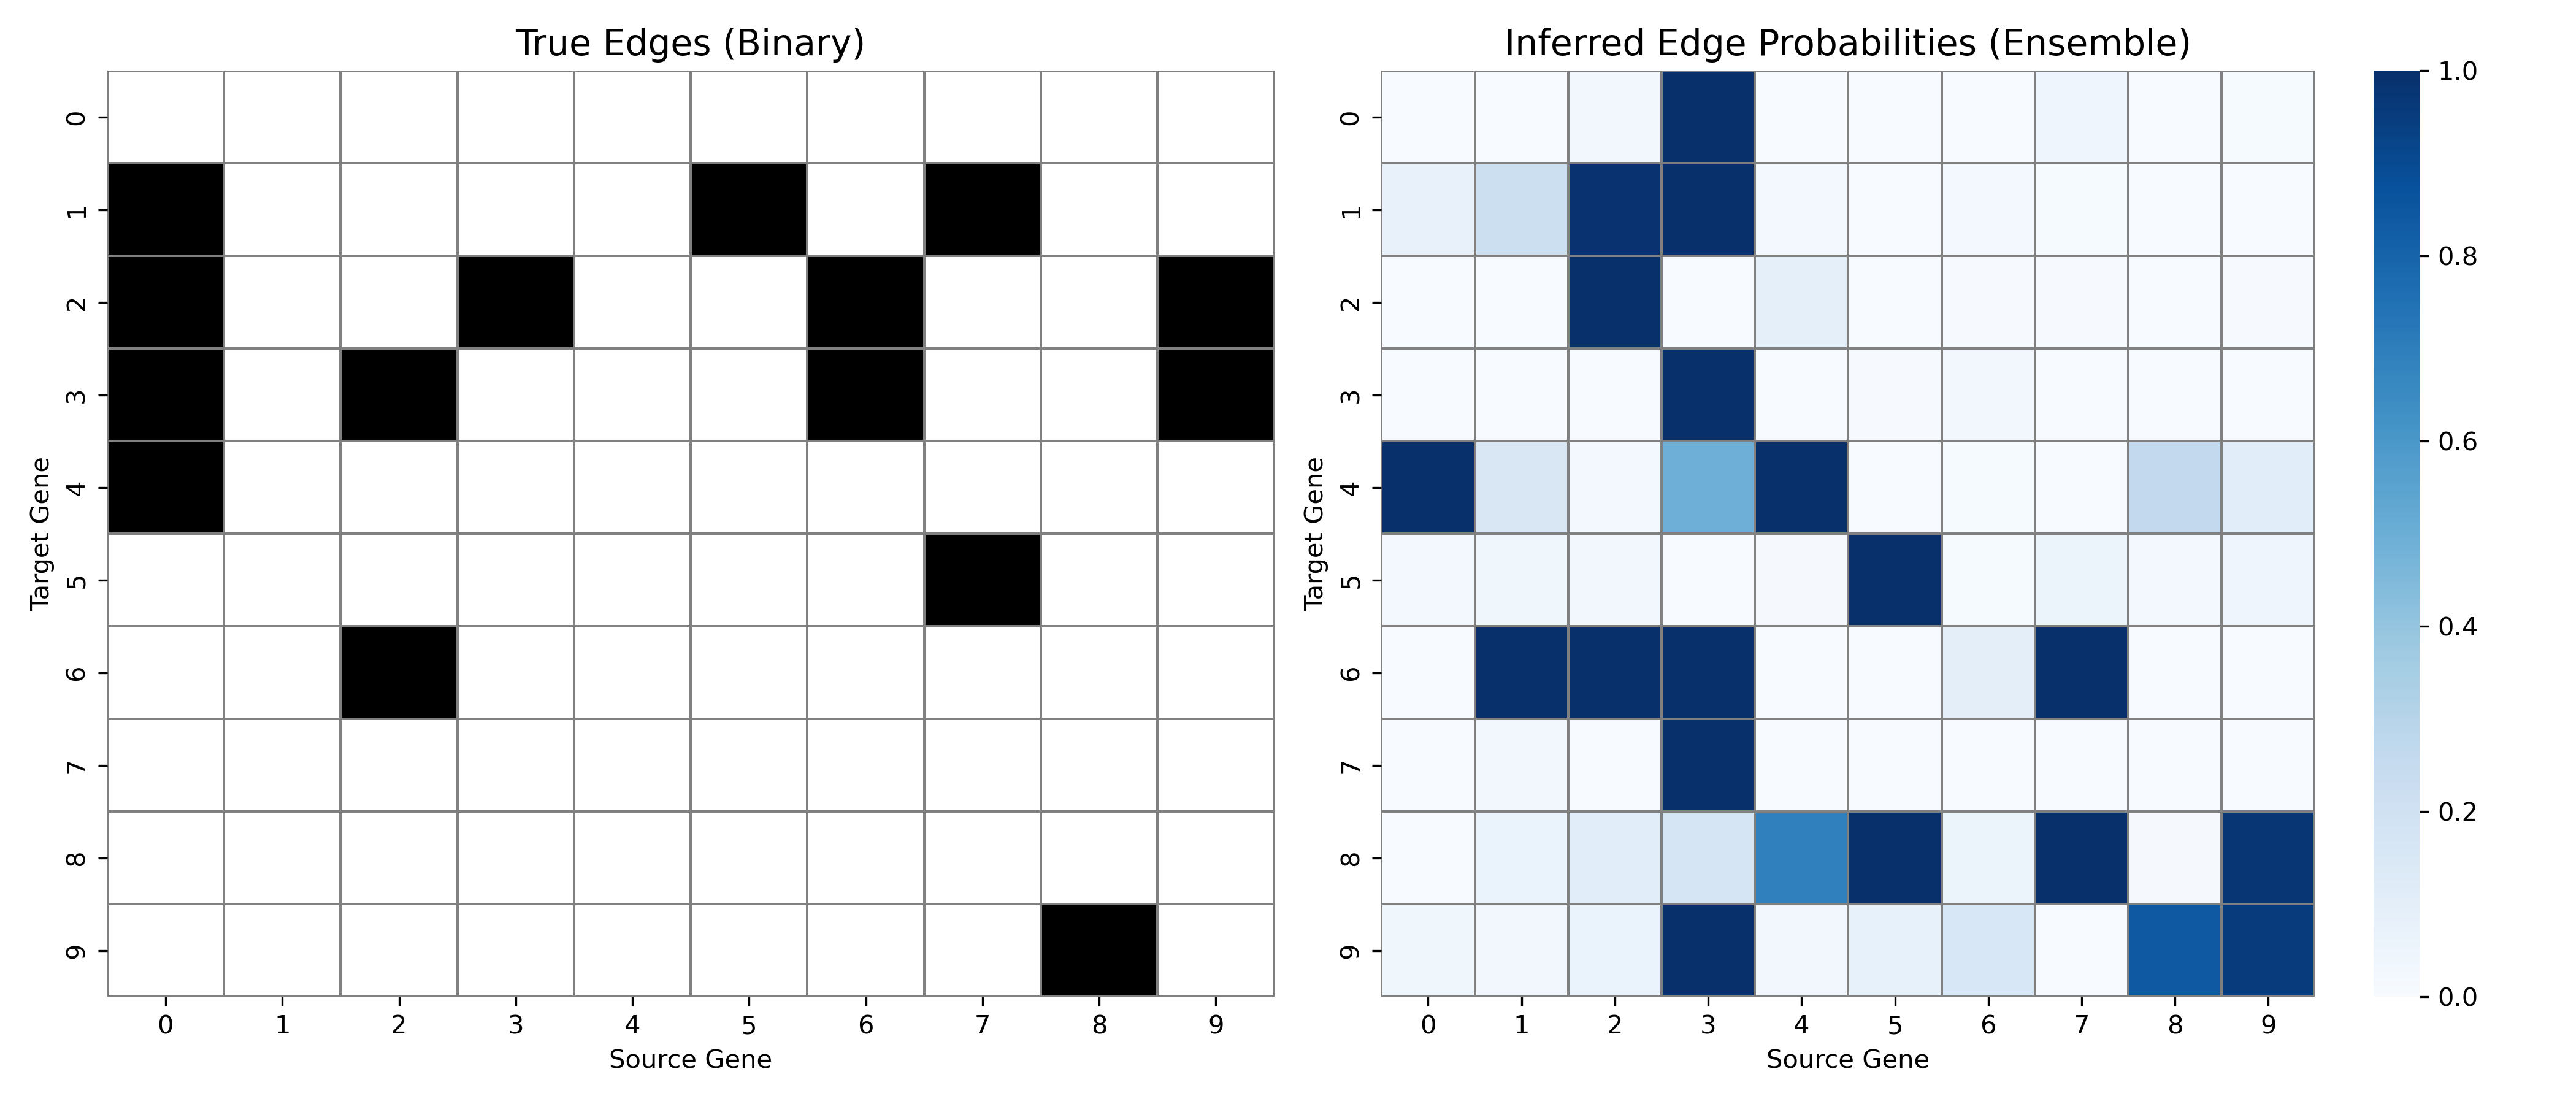
\includegraphics[width=0.8\textwidth]{../papers_figures/SM_dream4.png}
    \caption{\textbf{DREAM4 Inference Results.} Comparison between the true binary adjacency matrix (left) and the inferred marginal edge probabilities (right) for the DREAM4 10-node \textit{in silico} dataset. The homogeneous parameter constraint limits the structural recovery due to a mismatch with the highly heterogeneous thermodynamic model used to generate the DREAM4 data.}
    \label{fig:dream4}
\end{figure*}

\section{Baseline Competitor Hyperparameters}

To ensure a fair and reproducible benchmarking study against standard inference paradigms, the baseline methods were executed using the following settings:

\begin{itemize}
    \item \textbf{dynGENIE3:} Executed using the default Random Forest implementation tailored for time-series data. The number of trees was set to 1000 to ensure stable variable importance metrics.
    \item \textbf{Sparse ODE via Lasso (Inferelator-style):} Implemented as a regularized linear regression problem predicting the finite-difference derivative $\Delta x_i / \Delta t$. The $L_1$ regularization penalty ($\alpha$) was optimized independently for each node using 5-fold cross-validation (LassoCV) to enforce sparsity.
    \item \textbf{PySINDy:} The Sequential Thresholded Least Squares (STLSQ) optimizer was used. To remain comparable with our SDE model's capacity, the feature library was restricted to first-order polynomials (linear combinations of the node states). The sparsity threshold was optimized via cross-validation.
    \item \textbf{Granger Causality:} Executed using a classical Vector Autoregression (VAR) model. The optimal maximum lag was selected using the Akaike Information Criterion (AIC). F-tests were performed to determine the statistical significance of predictive causality, and the resulting p-values ($- \log_{10}(p)$) were used as confidence scores for the AUPRC evaluation.
\end{itemize}

$\tau \frac{dx_i}{dt} = -x_i + (1-x_i)\sigma\left(\sum_{j} W_{ij}x_j + I\right)$

\bibliographystyle{oup-abbrvnat}
\bibliography{reference}

\end{document}